% Options for packages loaded elsewhere
\PassOptionsToPackage{unicode}{hyperref}
\PassOptionsToPackage{hyphens}{url}
%
\documentclass[
]{article}
\usepackage{amsmath,amssymb}
\usepackage{lmodern}
\usepackage{iftex}
\ifPDFTeX
  \usepackage[T1]{fontenc}
  \usepackage[utf8]{inputenc}
  \usepackage{textcomp} % provide euro and other symbols
\else % if luatex or xetex
  \usepackage{unicode-math}
  \defaultfontfeatures{Scale=MatchLowercase}
  \defaultfontfeatures[\rmfamily]{Ligatures=TeX,Scale=1}
\fi
% Use upquote if available, for straight quotes in verbatim environments
\IfFileExists{upquote.sty}{\usepackage{upquote}}{}
\IfFileExists{microtype.sty}{% use microtype if available
  \usepackage[]{microtype}
  \UseMicrotypeSet[protrusion]{basicmath} % disable protrusion for tt fonts
}{}
\makeatletter
\@ifundefined{KOMAClassName}{% if non-KOMA class
  \IfFileExists{parskip.sty}{%
    \usepackage{parskip}
  }{% else
    \setlength{\parindent}{0pt}
    \setlength{\parskip}{6pt plus 2pt minus 1pt}}
}{% if KOMA class
  \KOMAoptions{parskip=half}}
\makeatother
\usepackage{xcolor}
\usepackage[margin=1in]{geometry}
\usepackage{color}
\usepackage{fancyvrb}
\newcommand{\VerbBar}{|}
\newcommand{\VERB}{\Verb[commandchars=\\\{\}]}
\DefineVerbatimEnvironment{Highlighting}{Verbatim}{commandchars=\\\{\}}
% Add ',fontsize=\small' for more characters per line
\usepackage{framed}
\definecolor{shadecolor}{RGB}{248,248,248}
\newenvironment{Shaded}{\begin{snugshade}}{\end{snugshade}}
\newcommand{\AlertTok}[1]{\textcolor[rgb]{0.94,0.16,0.16}{#1}}
\newcommand{\AnnotationTok}[1]{\textcolor[rgb]{0.56,0.35,0.01}{\textbf{\textit{#1}}}}
\newcommand{\AttributeTok}[1]{\textcolor[rgb]{0.77,0.63,0.00}{#1}}
\newcommand{\BaseNTok}[1]{\textcolor[rgb]{0.00,0.00,0.81}{#1}}
\newcommand{\BuiltInTok}[1]{#1}
\newcommand{\CharTok}[1]{\textcolor[rgb]{0.31,0.60,0.02}{#1}}
\newcommand{\CommentTok}[1]{\textcolor[rgb]{0.56,0.35,0.01}{\textit{#1}}}
\newcommand{\CommentVarTok}[1]{\textcolor[rgb]{0.56,0.35,0.01}{\textbf{\textit{#1}}}}
\newcommand{\ConstantTok}[1]{\textcolor[rgb]{0.00,0.00,0.00}{#1}}
\newcommand{\ControlFlowTok}[1]{\textcolor[rgb]{0.13,0.29,0.53}{\textbf{#1}}}
\newcommand{\DataTypeTok}[1]{\textcolor[rgb]{0.13,0.29,0.53}{#1}}
\newcommand{\DecValTok}[1]{\textcolor[rgb]{0.00,0.00,0.81}{#1}}
\newcommand{\DocumentationTok}[1]{\textcolor[rgb]{0.56,0.35,0.01}{\textbf{\textit{#1}}}}
\newcommand{\ErrorTok}[1]{\textcolor[rgb]{0.64,0.00,0.00}{\textbf{#1}}}
\newcommand{\ExtensionTok}[1]{#1}
\newcommand{\FloatTok}[1]{\textcolor[rgb]{0.00,0.00,0.81}{#1}}
\newcommand{\FunctionTok}[1]{\textcolor[rgb]{0.00,0.00,0.00}{#1}}
\newcommand{\ImportTok}[1]{#1}
\newcommand{\InformationTok}[1]{\textcolor[rgb]{0.56,0.35,0.01}{\textbf{\textit{#1}}}}
\newcommand{\KeywordTok}[1]{\textcolor[rgb]{0.13,0.29,0.53}{\textbf{#1}}}
\newcommand{\NormalTok}[1]{#1}
\newcommand{\OperatorTok}[1]{\textcolor[rgb]{0.81,0.36,0.00}{\textbf{#1}}}
\newcommand{\OtherTok}[1]{\textcolor[rgb]{0.56,0.35,0.01}{#1}}
\newcommand{\PreprocessorTok}[1]{\textcolor[rgb]{0.56,0.35,0.01}{\textit{#1}}}
\newcommand{\RegionMarkerTok}[1]{#1}
\newcommand{\SpecialCharTok}[1]{\textcolor[rgb]{0.00,0.00,0.00}{#1}}
\newcommand{\SpecialStringTok}[1]{\textcolor[rgb]{0.31,0.60,0.02}{#1}}
\newcommand{\StringTok}[1]{\textcolor[rgb]{0.31,0.60,0.02}{#1}}
\newcommand{\VariableTok}[1]{\textcolor[rgb]{0.00,0.00,0.00}{#1}}
\newcommand{\VerbatimStringTok}[1]{\textcolor[rgb]{0.31,0.60,0.02}{#1}}
\newcommand{\WarningTok}[1]{\textcolor[rgb]{0.56,0.35,0.01}{\textbf{\textit{#1}}}}
\usepackage{graphicx}
\makeatletter
\def\maxwidth{\ifdim\Gin@nat@width>\linewidth\linewidth\else\Gin@nat@width\fi}
\def\maxheight{\ifdim\Gin@nat@height>\textheight\textheight\else\Gin@nat@height\fi}
\makeatother
% Scale images if necessary, so that they will not overflow the page
% margins by default, and it is still possible to overwrite the defaults
% using explicit options in \includegraphics[width, height, ...]{}
\setkeys{Gin}{width=\maxwidth,height=\maxheight,keepaspectratio}
% Set default figure placement to htbp
\makeatletter
\def\fps@figure{htbp}
\makeatother
\setlength{\emergencystretch}{3em} % prevent overfull lines
\providecommand{\tightlist}{%
  \setlength{\itemsep}{0pt}\setlength{\parskip}{0pt}}
\setcounter{secnumdepth}{-\maxdimen} % remove section numbering
\ifLuaTeX
  \usepackage{selnolig}  % disable illegal ligatures
\fi
\IfFileExists{bookmark.sty}{\usepackage{bookmark}}{\usepackage{hyperref}}
\IfFileExists{xurl.sty}{\usepackage{xurl}}{} % add URL line breaks if available
\urlstyle{same} % disable monospaced font for URLs
\hypersetup{
  pdftitle={Tp Statistiques 2},
  pdfauthor={Lapu Matthias \textbar{} Amaël Kreis},
  hidelinks,
  pdfcreator={LaTeX via pandoc}}

\title{Tp Statistiques 2}
\author{Lapu Matthias \textbar{} Amaël Kreis}
\date{}

\begin{document}
\maketitle

\hypertarget{simulation-et-convergence}{%
\section{Simulation et convergence}\label{simulation-et-convergence}}

\hypertarget{i.-variation-sous-jacente-et-uxe9chantillonnage-ruxe9puxe9tuxe9}{%
\subsection{I. Variation sous-jacente et échantillonnage
répété}\label{i.-variation-sous-jacente-et-uxe9chantillonnage-ruxe9puxe9tuxe9}}

1.Si X ∼ \$\epsilon(0.5), quelle est la probabilité qu'on observe une
valeur supérieure à 3?

On a : \[ 
f(0.5) = 0.5e^{-0.5x} 
\] Donc pour : \[ 
X\sim\xi(0.5) 
\] On trouve: \[
P(X > 3)=
\int_{3}^{+\infty} \frac{1}{2}e^{\frac{-x}{2}}dx
= \left[-e^{-\frac{x}{2}}\right]_3^{+\infty}
=e^{-\frac{3}{2}}\approx0.223
\]

2.Simulez un échantillon de taille n = 20 d'un loi de \$\epsilon(0,5),
créez un histogramme de votre échantillon et commentez la forme de votre
histogramme. Superposer la vrai densité. Quelle est la probabilité
empirique qu'on observe une valeur supérieure à 3 ?

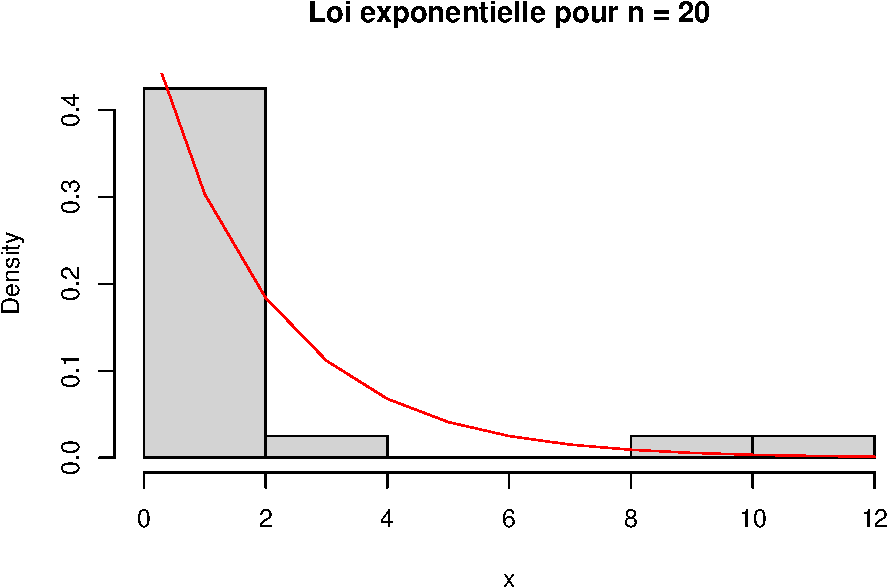
\includegraphics{tp2_files/figure-latex/q2-1.pdf}

\begin{verbatim}
## [1] "Ici P(X>3)= 0.1"
\end{verbatim}

L'histogramme peut être très proche de la densité ou au contraire s'en
éloigner énormément.

3.Répétez cette opération 5 ou 6 fois et commentez les différences entre
les histogrammes que vous obtenez à chaque fois. Utilisez la même limite
sur les axes pour faciliter la comparaison. Notez également comment la
probabilité empirique qu'on observe une valeur supérieure à 3 change.

\begin{verbatim}
## [1] "Echantillon  1  P(X>3)= 0.25"
## [1] "Echantillon  2  P(X>3)= 0.25"
## [1] "Echantillon  3  P(X>3)= 0.2"
## [1] "Echantillon  4  P(X>3)= 0.05"
## [1] "Echantillon  5  P(X>3)= 0.3"
## [1] "Echantillon  6  P(X>3)= 0.25"
\end{verbatim}

Les histogrammes sont tous très différent d'un échantillon a un autre,
cela est du a la faible taille des échantillons.

4.Augmentez la taille de votre échantillon à 100 et répétez votre
expérience. Que remarquez-vous?

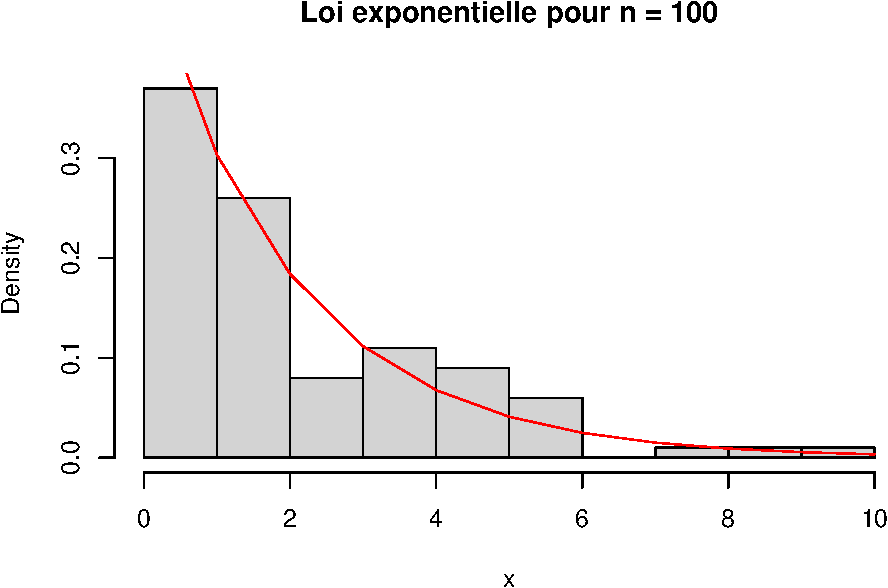
\includegraphics{tp2_files/figure-latex/unnamed-chunk-2-1.pdf}

On remarque que l'histogramme est bien plus proche de la densité que
précedement.

\hypertarget{ii.-variabilituxe9-aluxe9atoire-du-maximum-de-luxe9chantillon}{%
\subsection{II. Variabilité aléatoire du maximum de
l'échantillon}\label{ii.-variabilituxe9-aluxe9atoire-du-maximum-de-luxe9chantillon}}

1.Simuler un échantillon de taille n = 10 d'une loi U(−1, 1) et
enregistrez le maximum de l'échantillon.

\begin{Shaded}
\begin{Highlighting}[]
\NormalTok{loiU }\OtherTok{\textless{}{-}} \FunctionTok{runif}\NormalTok{(}\DecValTok{10}\NormalTok{, }\SpecialCharTok{{-}}\DecValTok{1}\NormalTok{, }\DecValTok{1}\NormalTok{)}
\NormalTok{max1 }\OtherTok{\textless{}{-}} \FunctionTok{max}\NormalTok{(loiU)}
\FunctionTok{print}\NormalTok{(max1)}
\end{Highlighting}
\end{Shaded}

\begin{verbatim}
## [1] 0.9233449
\end{verbatim}

2.Répétez les deux étapes ci-dessus dix fois, en écrivant le maximum de
l'échantillon à chaque fois. Commentez la variabilité des valeurs que
vous obtenez pour les maxima de votre échantillon.

\begin{Shaded}
\begin{Highlighting}[]
\NormalTok{max10 }\OtherTok{\textless{}{-}} \FunctionTok{c}\NormalTok{() }\CommentTok{\#création d\textquotesingle{}un vecteur vide}
\ControlFlowTok{for}\NormalTok{ (i }\ControlFlowTok{in} \DecValTok{1}\SpecialCharTok{:}\DecValTok{10}\NormalTok{) \{}
\NormalTok{  max10[i] }\OtherTok{=} \FunctionTok{max}\NormalTok{(}\FunctionTok{runif}\NormalTok{(}\DecValTok{10}\NormalTok{,}\SpecialCharTok{{-}}\DecValTok{1}\NormalTok{,}\DecValTok{1}\NormalTok{))}\CommentTok{\#chaque maximum est inséré à la position i du vecteur}
\NormalTok{\}}
\FunctionTok{print}\NormalTok{(max10)}
\end{Highlighting}
\end{Shaded}

\begin{verbatim}
##  [1] 0.9069923 0.9723631 0.6583771 0.9517615 0.9316664 0.9822200 0.8168893
##  [8] 0.7688478 0.9189602 0.8949810
\end{verbatim}

3.Répétez 100 fois et construisez un histogramme et une boîte à
moustaches. Quelle est la loi du maximum, M = max 1≤i≤n X i où X i ∼
U(−1, 1) (TD1) ? Superposer la densité théorique sur l'histogramme. Que
remarquez-vous ?

\begin{Shaded}
\begin{Highlighting}[]
\NormalTok{max100 }\OtherTok{\textless{}{-}} \FunctionTok{c}\NormalTok{() }
\ControlFlowTok{for}\NormalTok{(i }\ControlFlowTok{in} \DecValTok{1}\SpecialCharTok{:}\DecValTok{100}\NormalTok{)\{}
\NormalTok{ max100[i] }\OtherTok{=} \FunctionTok{max}\NormalTok{(}\FunctionTok{runif}\NormalTok{(}\DecValTok{10}\NormalTok{,}\SpecialCharTok{{-}}\DecValTok{1}\NormalTok{,}\DecValTok{1}\NormalTok{)) }
\NormalTok{\}}
\FunctionTok{hist}\NormalTok{(max100,}\AttributeTok{breaks=}\DecValTok{10}\NormalTok{,}\AttributeTok{main =} \StringTok{"Histogramme du maximum de la loi uniforme n=10"}\NormalTok{, }\AttributeTok{freq =} \ConstantTok{FALSE}\NormalTok{)}
\NormalTok{densitermax100 }\OtherTok{\textless{}{-}} \FunctionTok{density}\NormalTok{(max100) }\CommentTok{\#cette fonction permet d\textquotesingle{}obtenir la densité de la loi}
\FunctionTok{lines}\NormalTok{(densitermax100,}\AttributeTok{lwd=}\DecValTok{2}\NormalTok{,}\AttributeTok{col=}\StringTok{"red"}\NormalTok{) }\CommentTok{\#superposition de la densité i}
\end{Highlighting}
\end{Shaded}

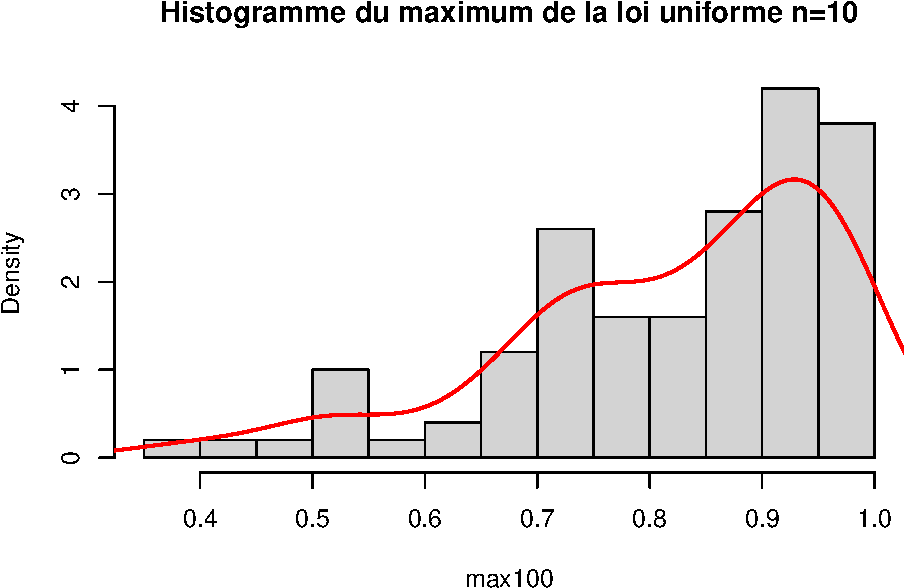
\includegraphics{tp2_files/figure-latex/unnamed-chunk-5-1.pdf}

\begin{Shaded}
\begin{Highlighting}[]
\FunctionTok{boxplot}\NormalTok{(max100, }\AttributeTok{horizontal =} \ConstantTok{TRUE}\NormalTok{)}
\end{Highlighting}
\end{Shaded}

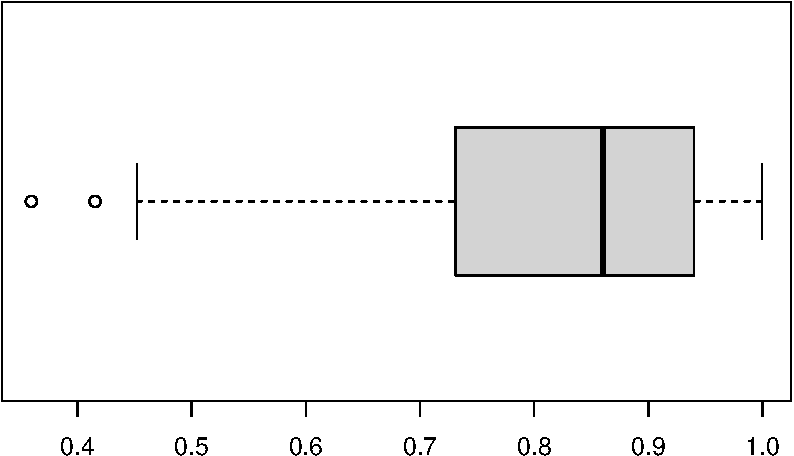
\includegraphics{tp2_files/figure-latex/unnamed-chunk-5-2.pdf} On
remarque que la densité est très proche des maximums obtenues.

On cherche à déterminer la loi du maximum d'un échantillon de loi
uniforme : \[
F_M(x) = P(M \le x) = P(max(X_i) \le x) 
\\
= P(\bigl\{X_1 \le x \bigl\} \cap \bigl\{ X_2 \le x\bigl\} ... \bigl\{ X_n \le x\bigl\})
\] Par indépendance des \$X\_i \[
 = \prod_{i=1}^n P(X_i \le x)
\] Car les \$X\_i sont identiquement distribués, ils possèdent la même
loi donc la même fonction de répartition.

\[
= (F_{X_1}(x))^n
\] La loi du maximum, lorsque \$X \in [a;b] est donc : \[
(\frac{x-a}{b-a})^n
\] 4.Augmentez la taille de votre échantillon à 50 et répétez votre
expérience. Que remarquez-vous? Sont-ils proches de la symétrie ?

\begin{Shaded}
\begin{Highlighting}[]
\NormalTok{max100loi50 }\OtherTok{\textless{}{-}} \FunctionTok{c}\NormalTok{()}
\ControlFlowTok{for}\NormalTok{(i }\ControlFlowTok{in} \DecValTok{1}\SpecialCharTok{:}\DecValTok{100}\NormalTok{)\{}
\NormalTok{  max100loi50[i] }\OtherTok{\textless{}{-}} \FunctionTok{max}\NormalTok{(}\FunctionTok{runif}\NormalTok{(}\DecValTok{50}\NormalTok{, }\SpecialCharTok{{-}}\DecValTok{1}\NormalTok{, }\DecValTok{1}\NormalTok{))}
\NormalTok{\}}
\FunctionTok{hist}\NormalTok{(max100loi50,}\AttributeTok{breaks=}\DecValTok{10}\NormalTok{, }\AttributeTok{main =} \StringTok{"Histogramme du maximum de la loi uniforme n=50"}\NormalTok{, }\AttributeTok{freq =} \ConstantTok{FALSE}\NormalTok{)}
\FunctionTok{lines}\NormalTok{(}\FunctionTok{density}\NormalTok{(max100loi50),}\AttributeTok{lwd=}\DecValTok{2}\NormalTok{,}\AttributeTok{col=}\StringTok{"red"}\NormalTok{)}
\end{Highlighting}
\end{Shaded}

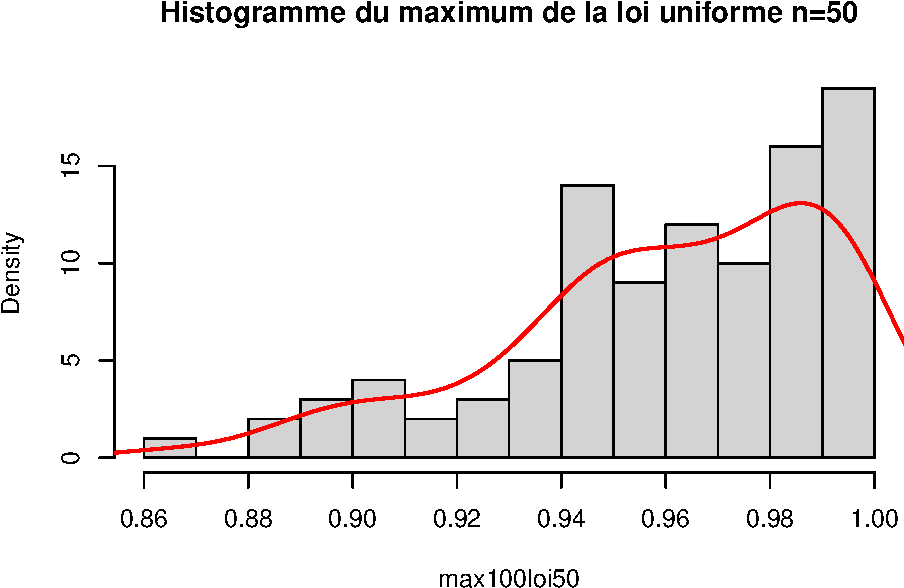
\includegraphics{tp2_files/figure-latex/unnamed-chunk-6-1.pdf}

\begin{Shaded}
\begin{Highlighting}[]
\FunctionTok{boxplot}\NormalTok{(max100, }\AttributeTok{horizontal =} \ConstantTok{TRUE}\NormalTok{)}
\end{Highlighting}
\end{Shaded}

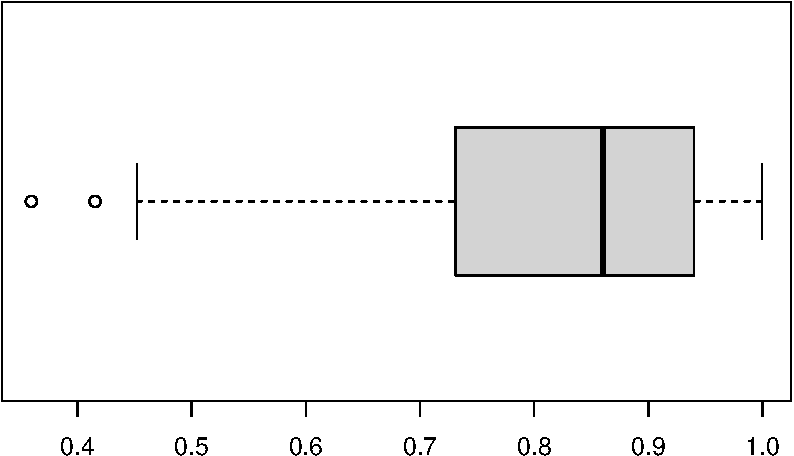
\includegraphics{tp2_files/figure-latex/unnamed-chunk-6-2.pdf} Ils ne
semble pas particulièrement plus proche de la symétrie. \# Monte Carlo
Methods

Vérifier que : \[
E[\hat{\theta}] = \theta
\] Nous utiliserons la linéarité de l'espérance : \[
E[\frac{1}{n} \sum_{i=1}^{n} \psi(X)] = \frac{1}{n} \sum_{i=1}^n E[\psi(X)] = \frac{1}{n}*n*\theta=\theta
\] \#\# Moyenne et phénomène de concentration.

1.Donner une borne de cette quantité en utilisant l'inégalité de
Bienaymé Chebychev.

Rappelons l'inégalité de Bienaymé Chebychev : \[
P(| \hat{\theta}-\theta| \ge \delta) \le \frac{V(\hat{\theta})}{\delta²}
\]

Calculons la variance de cette quantité grâce au caractère quadratique
de la variance ainsi qu'à l'indépendance des \$X\_i : \[
V(\hat{\theta}) = V(\frac{1}{n} \sum_{i=1}^{n} \psi(X)) = \frac{1}{n²}V(\sum_{i=1}^n \psi(X)) = \frac{1}{n²} \sum_{i=1}^n V(\psi(X)) = \frac{1}{n²} *n\sigma² = \frac{\sigma²}{n}
\] On retrouve donc une borne pour cette inégalité.

\[
P(|\hat{\theta} - \theta| \ge \delta) \le \frac{\sigma²}{n\delta²}
\] 2. En supposant que a ≤ ψ(Xi) ≤ b, donner une borne en utilisant
l'inégalité de Hoeffding.

Posons : \[
S_{n} = \sum_{k=1}^n \psi(X_k)
\] D'après l'énoncé, nous savons que : \[
\frac{1}{n} \sum_{i=1}^n \psi(X_i) = \hat{\theta}
\] Ainsi : \[
\frac{S_n}{n} = \hat{\theta} 
\] Donc : \[
S_n=n\hat{\theta}
\]

D'après l'inégalité de Hoeffding nous savons que : \[
P(|S_n - E(S_n)| \geq t) \leq 2exp(\frac{-2t²}{\sum_{k=1}^n (b_k-a_k)²})
\]

Calculons l'esperance de S\_n: \[
E(S_n) = E(\sum_{k=1}^n \psi(X_k)) = \sum_{k=1}^n E(\psi(X_k)) = \sum_{k=1}^n \theta = n\theta
\] Ainsi : \[
P(|n\hat{\theta} - n\theta| \geq t) \leq 2exp(\frac{-2t²}{\sum_{k=1}^n (b_k-a_k)²})
\\
P(|\hat{\theta} - \theta| \geq \frac{t}{n}) \leq 2exp(\frac{-2t²}{\sum_{k=1}^n (b_k-a_k)²})
\]

On pose : \[
\frac{t}{n} = \delta
\\
P(|\hat{\theta} - \theta| \geq \delta) \leq 2exp(\frac{-(2n\delta)²}{\sum_{k=1}^n (b_k-a_k)²})
\] 3. De combien d'échantillons auriez-vous besoin pour que la
probabilité que \delta = 2\phi soit inférieur à 1\%.

Servons-nous de l'inégalité de Bienaymé-Tchebychev que nous avons trouvé
lors du 1.

\[
P(|\hat{\theta} - \theta| \ge \delta) \le \frac{\sigma²}{n\delta²}
\] Remplaçons par : \[
\delta = 2\sigma
\\
\delta²=4\sigma²
\] Ainsi : \[
\frac{\sigma²}{n\delta²} = \frac{1}{4n}
\] Or l'énoncé demande à ce que la probabilité soit inférieur à 1\% ,
c'est-à-dire que : \[
\frac{1}{4n} = 0.01  \Longrightarrow n=25
\] Afin que la probabilité soit inférieur à 1\%, il faut 25
échantillons.

\hypertarget{application-pour-lestimation-de-probabilituxe9}{%
\subsection{Application pour l'estimation de
probabilité}\label{application-pour-lestimation-de-probabilituxe9}}

\begin{enumerate}
\def\labelenumi{\arabic{enumi}.}
\tightlist
\item
  Pour la question I avec E(0.5), identifier le paramètre d'intérêt θ et
  donner un estimateur θ̂.
\end{enumerate}

On cherche un estimateur pour la loi exponentielle. En prenant un
échantillon : \[
(X_1,X_2,...,X_n)
\] \[
X_i \sim \varepsilon(\theta) 
\\
\forall \theta \in R^*_+
\\
E[X_i] = \frac{1}{\theta}
\\
\bar{X} = \frac{1}{n} \sum_{i=1}^{n} X_i
\] La moyenne empirique tend presque surement vers l'estimateur. Ainsi :
\[
\hat{\theta}_n = \frac{1}{\bar{X}}
\] 2. Utilisons l'inégalité de Hoeffding.

L'énoncé demande à ce que E(Z) = garantie probabiliste de l'erreur. Il
faut trouver Z .

On pose : \[
Z = 1_{|\hat{\theta} - \theta| \ge \delta} 
\] Ainsi, nous avons donc : \[
\eta = P(|\hat{\theta} - \theta| \ge \delta) = E[Z]
\] D'après la méthode de Monte Carlo, on a donc : \[
\eta \approx  \frac{1}{n} \sum_{i=1}^n Z_i
\]

\hypertarget{thuxe9oruxe8me-central-limite-et-estimation-monte-carlo}{%
\section{Théorème Central Limite et Estimation Monte
Carlo}\label{thuxe9oruxe8me-central-limite-et-estimation-monte-carlo}}

1. Vérifier que l'espérance théorique d'une loi de Pareto est E {[}X{]}
= αa/α−1.

\[
P(X\le t)= (1-\left( \frac{a}{t} \right)^{\alpha}) , \;avec \;x \ge a
\]

Donc : \[
E(X) = \int_0^{+\infty} 1-P(X \le t)dt =
\int_0^{+\infty} P(X    > t) dt =
a+a^{\alpha}\int_a^{+\infty}\frac{1}{t^{\alpha}}dt=a + \frac{a}{\alpha -1} =
\frac{\alpha a}{\alpha -1}
\]

2 et 3 . Simuler N = 1000 échantillons i.i.d de loi commune Pareto P(a,
α) (avec votre choix de paramètres) de taille n = 5, 30, 100 et calculer
les moyennes et variances empiriques ¯Xn,i et Sn,i, i = 1, . . . ,N.
Puis tracer l'histogramme des moyennes empiriques.

On prend \[ a = 1, \alpha = 3 \]

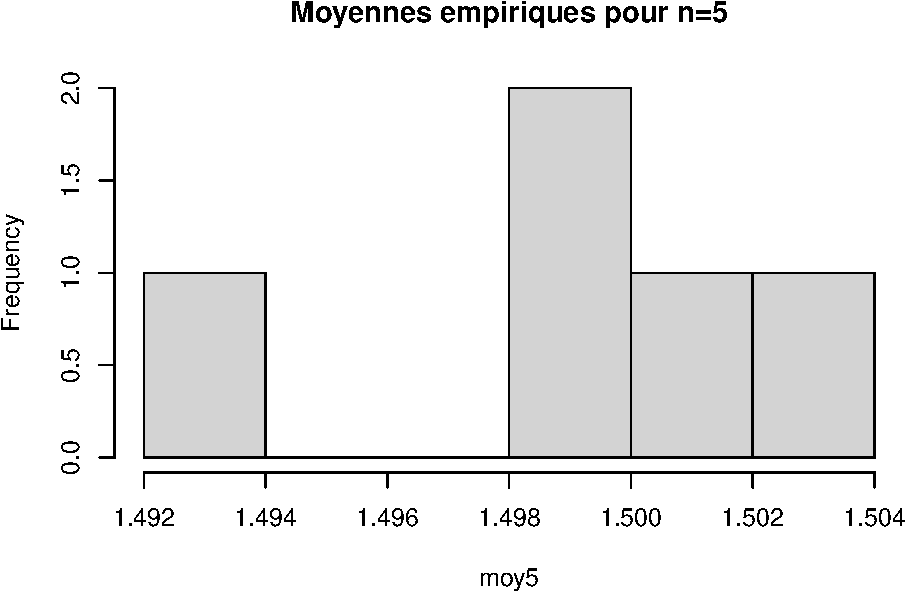
\includegraphics{tp2_files/figure-latex/echantillons-1.pdf}
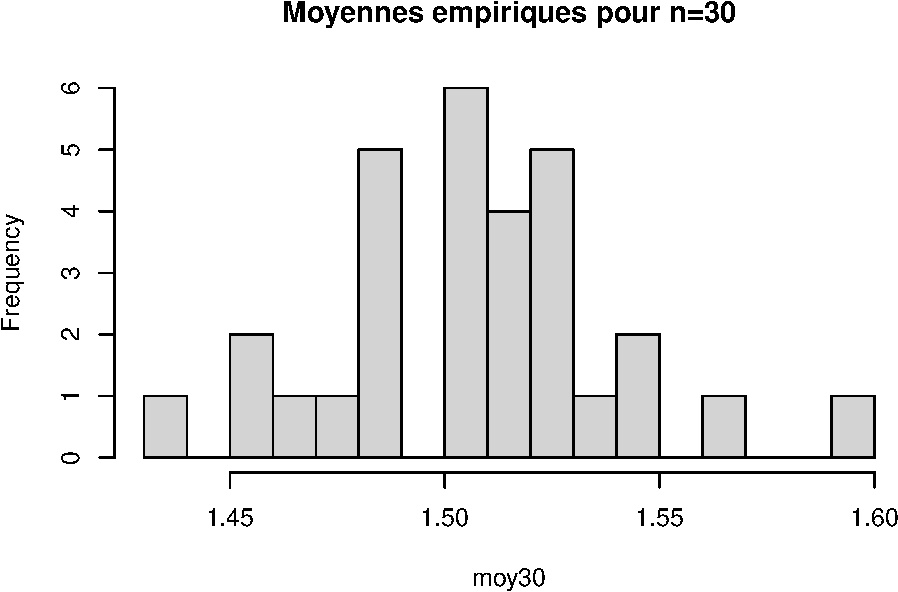
\includegraphics{tp2_files/figure-latex/echantillons-2.pdf}
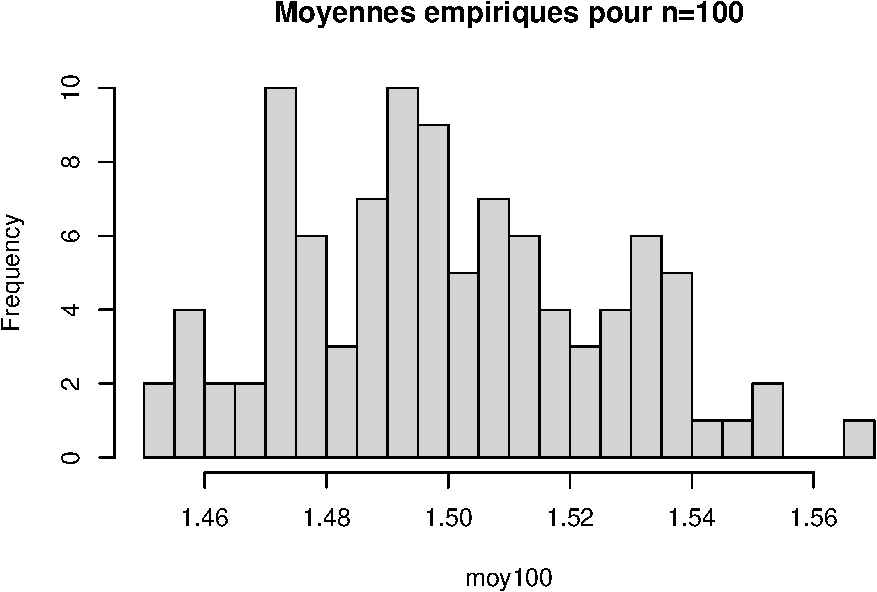
\includegraphics{tp2_files/figure-latex/echantillons-3.pdf}

\begin{enumerate}
\def\labelenumi{\arabic{enumi}.}
\setcounter{enumi}{3}
\tightlist
\item
  A l'aide d'une renormalisation adéquate (an, bn), montrer que Un,i =
  ¯Xn,i−an/ bn a une loi que vous pouvez approchez. Comparez histogramme
  de les moyennes empiriques normalisées, Un,i, et distribution
  théorique approchée. Quelle est l'influence de la taille de
  l'échantillon n sur la qualité de cette approximation?
\end{enumerate}

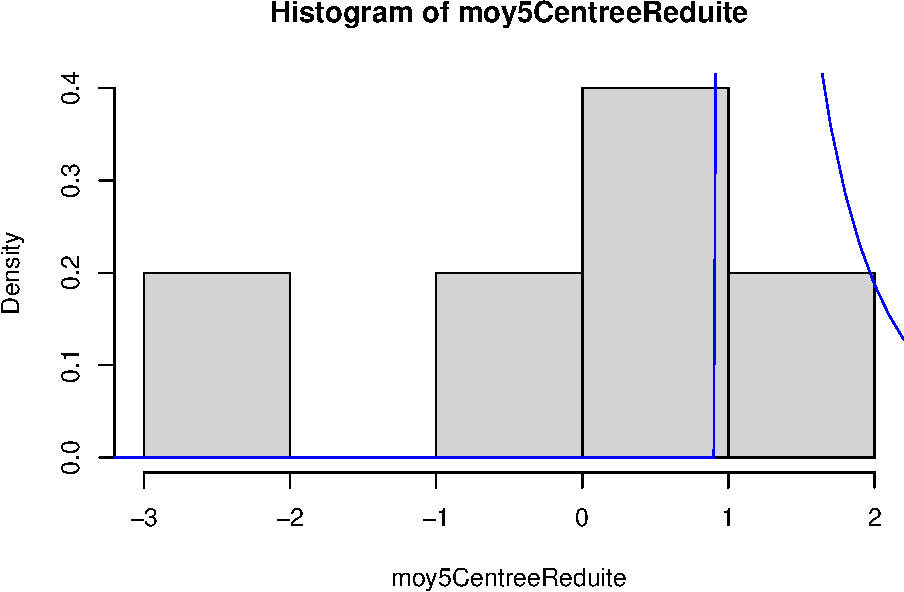
\includegraphics{tp2_files/figure-latex/normalisation-1.pdf}
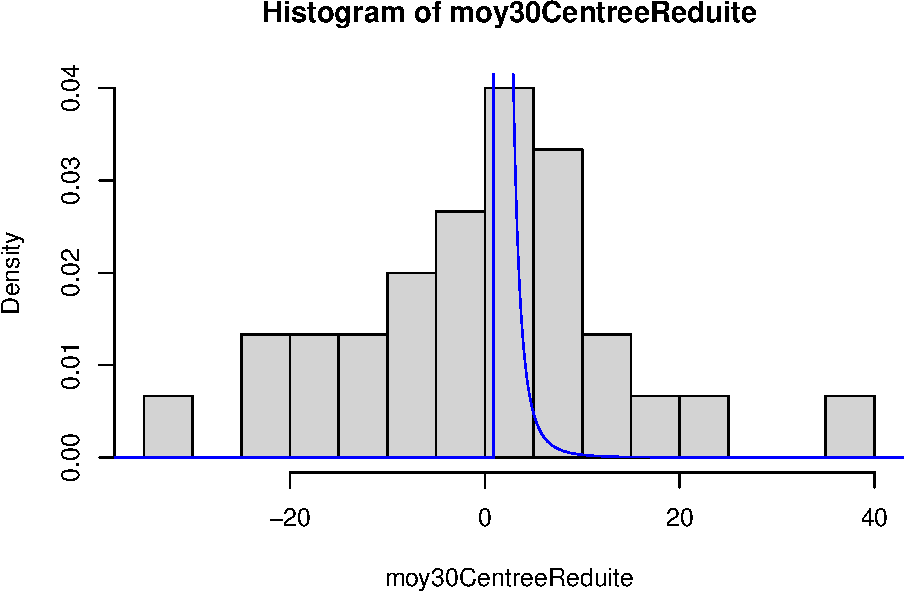
\includegraphics{tp2_files/figure-latex/normalisation-2.pdf}
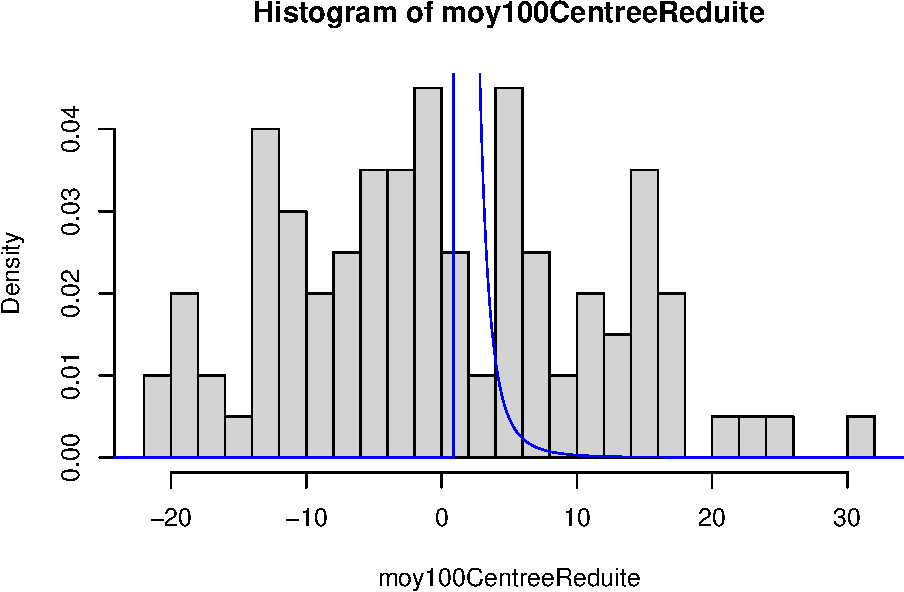
\includegraphics{tp2_files/figure-latex/normalisation-3.pdf}

\hypertarget{quand-le-thuxe9oruxe8me-de-central-limite-ne-sapplique-pas}{%
\subsection{Quand le théorème de central limite ne s'applique
pas}\label{quand-le-thuxe9oruxe8me-de-central-limite-ne-sapplique-pas}}

1. Simuler un échantillon de taille n = 20 d'une loi de C(2) et calculer
la moyenne empirique ¯Xn.

Cauchy20 est une simulation d'un échantillon n=20.

\begin{verbatim}
## [1] -1.292373
\end{verbatim}

2. Faites varier la taille de l'échantillon n = 20, 100, 1000 et 10000.
Qu'en déduire ?

\begin{verbatim}
## [1] -1.292373
\end{verbatim}

\begin{verbatim}
## [1] 18.93397
\end{verbatim}

\begin{verbatim}
## [1] 2.717784
\end{verbatim}

\begin{verbatim}
## [1] -1.691469
\end{verbatim}

On remarque que malgré le nombre élévé de l'échantillon la moyenne ne
semble pas se stabiliser comme pour une loi normale.

3. Expliquer ce comportement

Nous savons d'après le cours de probabilités que la loi de cauchy
n'admet pas d'espérance ni d'écart type. Cela explique donc le
comportement de la moyenne malgré la taille de l'échantillon.

4. Quelle est la médiane d'une loi de cauchy ?

La courbe est symétrique ,la médiane d'une loi de cauchy est \theta.
D'après le manuel de R, quand la position n'est pas défini celle-ci est
mise à 0. Par conséquent nous devons vérifier si la médiane semble
proche de 0.

\[
f(x,\theta) = \frac{1}{\pi} \frac{1}{1 + (x-\theta)²}
\frac{1}{2} = \frac{1}{\pi} \int_{-a}^{a} \frac{dx}{1+(x-\theta)²}
F^{-1} (\frac{1}{2}) = \theta
\]

5. En déduire un estimateur de theta et evaluer la performance de cet
estimateur sur les différents échantillons.

Nous pouvons essayer d'approximer theta , c'est-à-dire la médiane, cela
revient donc à chercher une estimation du quantile en 0.5 . D'après le
cours, les quantiles permettent de localiser les valeurs les plus
fréquentes. Nous allons donc essayer d'estimer le quantile.

\begin{Shaded}
\begin{Highlighting}[]
\FunctionTok{hist}\NormalTok{(cauchy20,}\AttributeTok{breaks=}\DecValTok{20}\NormalTok{)}
\FunctionTok{abline}\NormalTok{(}\AttributeTok{v=}\FunctionTok{mean}\NormalTok{(cauchy20),}\AttributeTok{col=}\StringTok{"red"}\NormalTok{,}\AttributeTok{lwd=}\DecValTok{3}\NormalTok{)}
\end{Highlighting}
\end{Shaded}

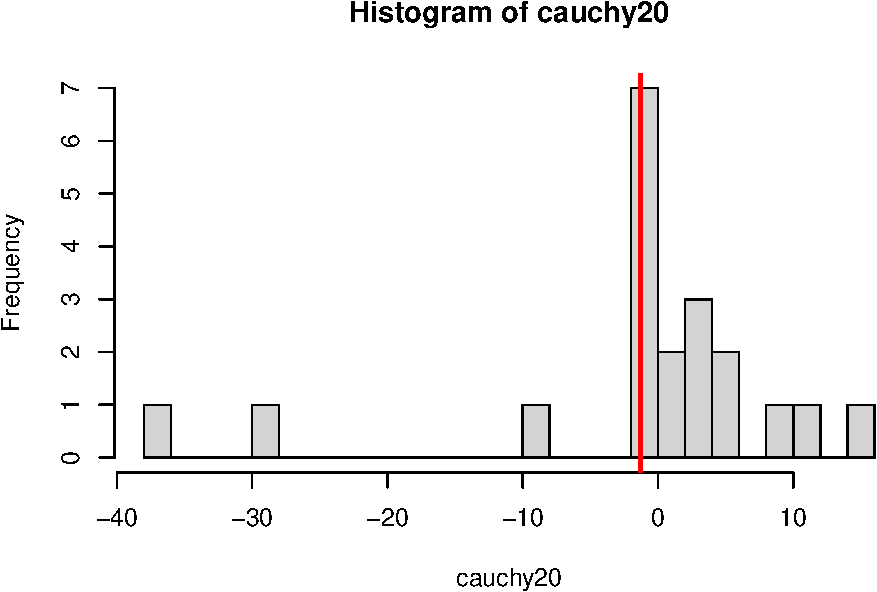
\includegraphics{tp2_files/figure-latex/unnamed-chunk-9-1.pdf}

\begin{Shaded}
\begin{Highlighting}[]
\FunctionTok{hist}\NormalTok{(cauchy100,}\AttributeTok{breaks=}\DecValTok{100}\NormalTok{)}
\FunctionTok{abline}\NormalTok{(}\AttributeTok{v=}\FunctionTok{mean}\NormalTok{(cauchy100),}\AttributeTok{col=}\StringTok{"red"}\NormalTok{,}\AttributeTok{lwd=}\DecValTok{3}\NormalTok{)}
\end{Highlighting}
\end{Shaded}

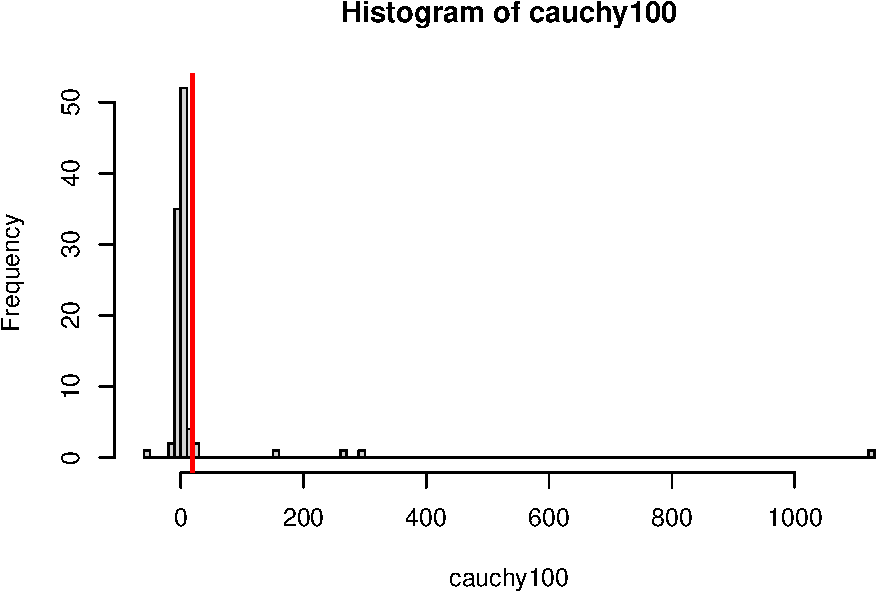
\includegraphics{tp2_files/figure-latex/unnamed-chunk-9-2.pdf}

\begin{Shaded}
\begin{Highlighting}[]
\FunctionTok{hist}\NormalTok{(cauchy1000,}\AttributeTok{xlim=}\FunctionTok{c}\NormalTok{(}\SpecialCharTok{{-}}\DecValTok{100}\NormalTok{,}\DecValTok{100}\NormalTok{),}\AttributeTok{breaks=}\DecValTok{1000}\NormalTok{)}
\FunctionTok{abline}\NormalTok{(}\AttributeTok{v=}\FunctionTok{mean}\NormalTok{(cauchy1000),}\AttributeTok{col=}\StringTok{"red"}\NormalTok{,}\AttributeTok{lwd=}\DecValTok{3}\NormalTok{)}
\end{Highlighting}
\end{Shaded}

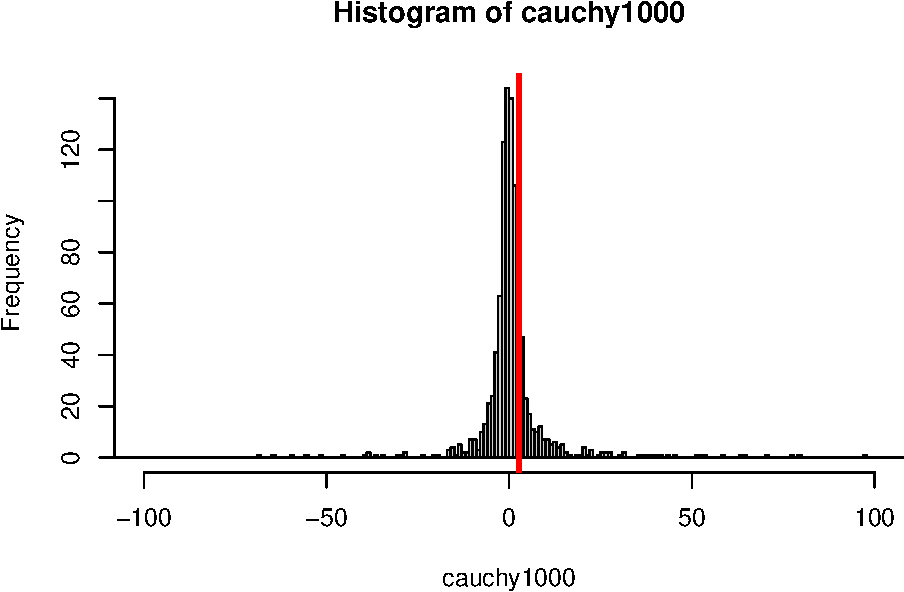
\includegraphics{tp2_files/figure-latex/unnamed-chunk-9-3.pdf}

\begin{Shaded}
\begin{Highlighting}[]
\FunctionTok{hist}\NormalTok{(cauchy10000,}\AttributeTok{xlim=}\FunctionTok{c}\NormalTok{(}\SpecialCharTok{{-}}\DecValTok{100}\NormalTok{,}\DecValTok{100}\NormalTok{),}\AttributeTok{breaks=}\DecValTok{10000}\NormalTok{)}
\FunctionTok{abline}\NormalTok{(}\AttributeTok{v=}\FunctionTok{mean}\NormalTok{(cauchy10000),}\AttributeTok{col=}\StringTok{"red"}\NormalTok{,}\AttributeTok{lwd=}\DecValTok{3}\NormalTok{)}
\end{Highlighting}
\end{Shaded}

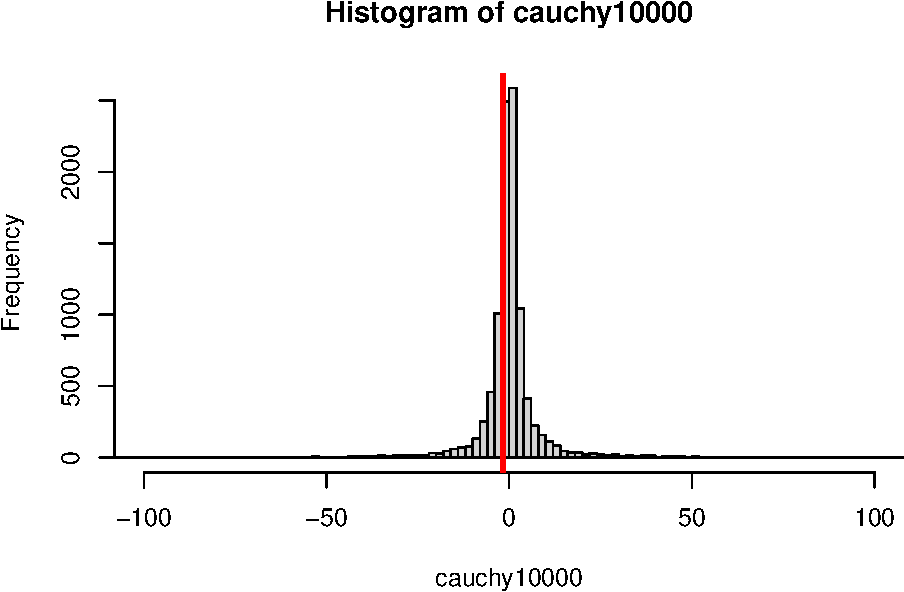
\includegraphics{tp2_files/figure-latex/unnamed-chunk-9-4.pdf}

D'après les graphiques nous pouvons remarquer que l'estimation de theta
semble proche de la vrai valeur, n'ayant pas de moyen de calculer
l'espérance de la loi cela semble être un bon estimateur, car celui-ci
semble proche de 0, assez pour jugé les performances de cet estimateur
comme suffisant.

\end{document}
